\section{PI szabályzó tervezése}

%{{{ Bevezetés, értelmezés

Ebben a feladatban a motorra egy PI szabályzót kapcsolunk, melynek átviteli függvénye
\begin{equation}
	\fn{W}_\text{c} = P\brc{1+\frac{1}{T_\text{I}s}},
\end{equation}
valamint a rendszer hatásvázlatát \aref{fig:pi-hatasvazlat}. ábra mutatja.

\begin{figure}[H]
	\centering
	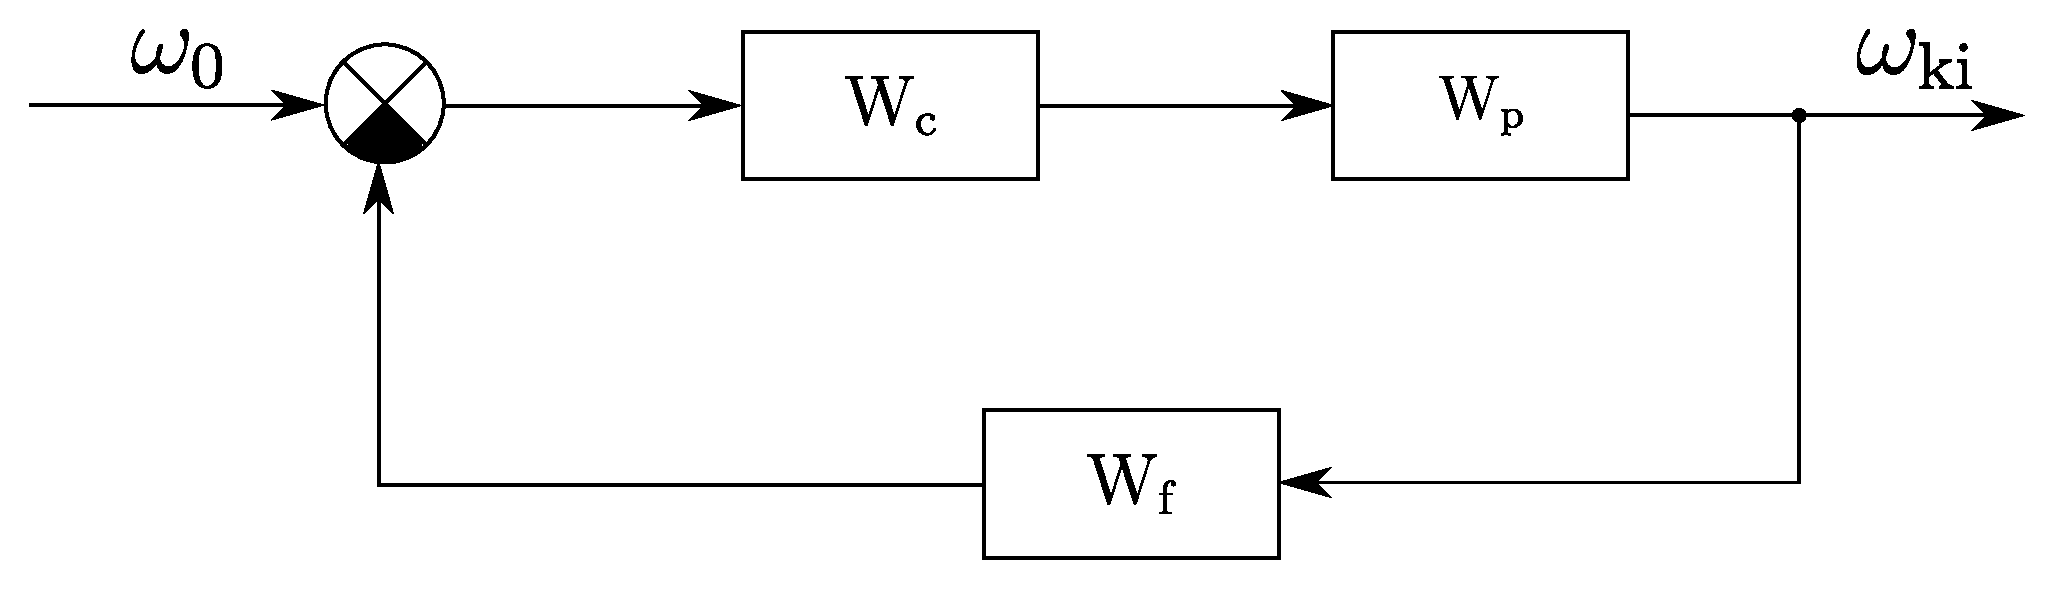
\includegraphics[width=.6\textwidth]{pi-hatasvazlat}
	\caption{PI-szabályozott rendszer hatásvázlata}
	\label{fig:pi-hatasvazlat}
\end{figure}

A motort egyetlen átviteli függvénnyel írjuk le, 
\aref{fig:process-hatasvazlat}. ábrának megfelelően.
Ezt irányított szakasznak hívjuk, és kifejtve a
\begin{equation}
	\fn{W}_\text{p} = \fn{W}_{\fn{U}_0\rightarrow\Omega_\text{ki}} =
	\frac{\km}{\Ja\, \La\, s^2 + \Ja\, \Ra\, s + \ke\, \km}
\end{equation}
alakot kapja.
A visszacsatoló ág üres, tehát $\fn{W}_\text{f} = 1$.

\begin{figure}[H]
	\centering
	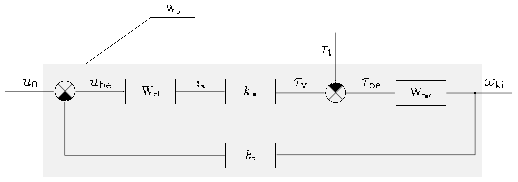
\includegraphics[width=.8\textwidth]{process-hatasvazlat}
	\caption{A motor átviteli függvénye $\fn{W}_\text{p}$}
	\label{fig:process-hatasvazlat}
\end{figure}

Az integráló tag időállandóját a szabályozott szakasz legnagyobb időállandójával
tesszük egyenlővé. Ez \aref{eq:T1}. egyenlet alapján $T_1 = 0,0145$ s.

%}}}

%{{{ A zárt szabályozási kör egyenletei
\subsection{A zárt szabályozási kör egyenletei}

Jelöljük az előrevezető ág átviteli függvényét $\fn{W}_\text{x}$-val.
A zárt szabályozási kör átviteli függvénye
\begin{equation}\label{eq:W-x}
	\fn{W}_\text{o} = \frac{\fn{W}_\text{x}}{1 + \fn{W}_\text{x}} =
	\frac{P\, \km\, \left(T_\text{I}\, s + 1\right)}{P\, \km + \Ja\, \La\, T_\text{I}\, s^3 + \Ja\, \Ra\, T_\text{I}\, s^2 + P\, T_\text{I}\, \km\, s + T_\text{I}\, \ke\, \km\, s}
\end{equation}

A zárt szabályozási kör karakterisztikus egyenlete \aref{eq:W-x}. egyenlet nevezője, 
ami nullával egyenlő.
\begin{equation}
	P\, \km + \Ja\, \La\, T_\text{I}\, s^3 + \Ja\, \Ra\, T_\text{I}\, s^2 + P\, T_\text{I}\, \km\, s + T_\text{I}\, \ke\, \km\, s = 0
\end{equation}
%}}}

%{{{ Stabilitás a P függvényében
\subsection{Stabilitás a körerősítés függvényében}

Rajzoljuk ki a pólusok valós részeit a körerősítés függvényében.
\Aref{fig:poles}. ábrán jól látszik, hogy minden pozitív $P$ értékre a pólusok
negatív része valós, tehát a rendszer stabil.
\begin{figure}[H]
	\centering
	\begin{subfigure}{.49\textwidth}
		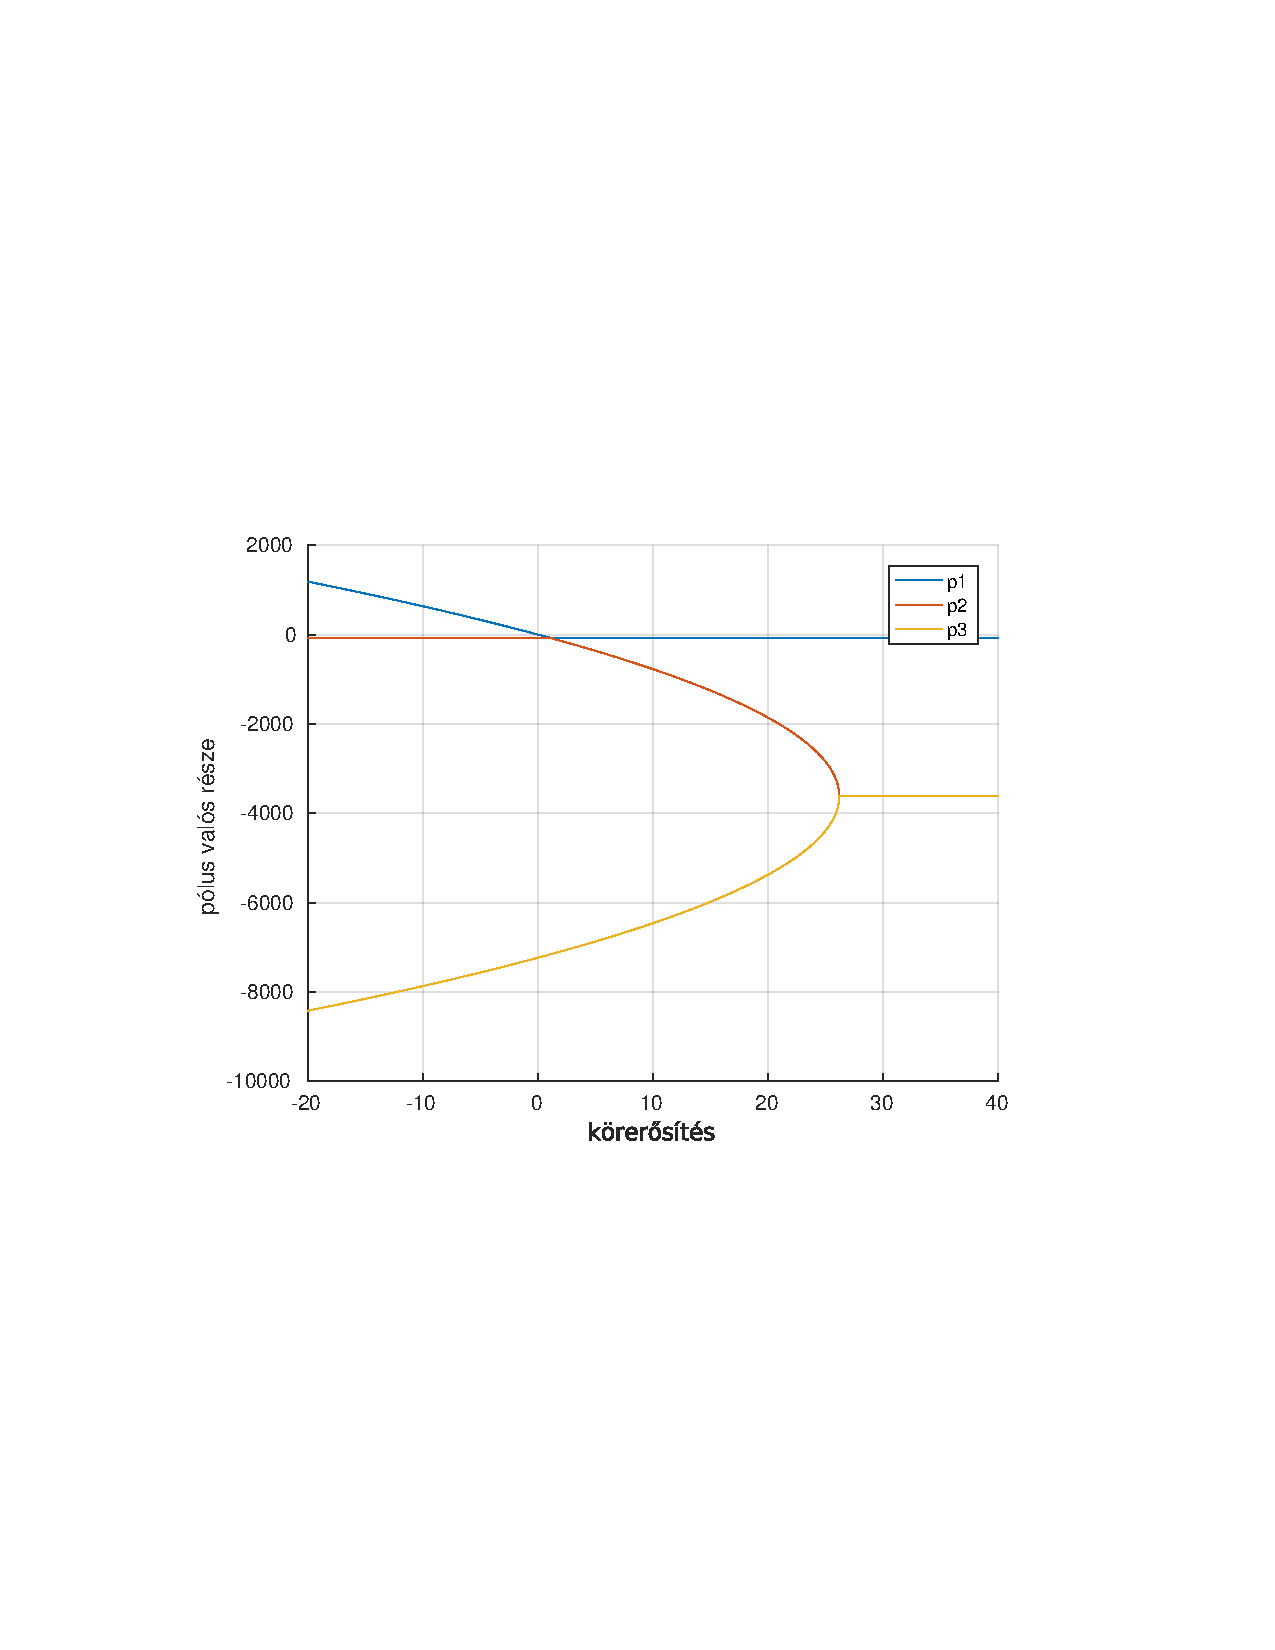
\includegraphics[width=\linewidth, trim=90 240 100 242, clip]{polus}
		\caption{Lényeges $P$ értékek}
	\end{subfigure}
	\begin{subfigure}{.49\textwidth}
		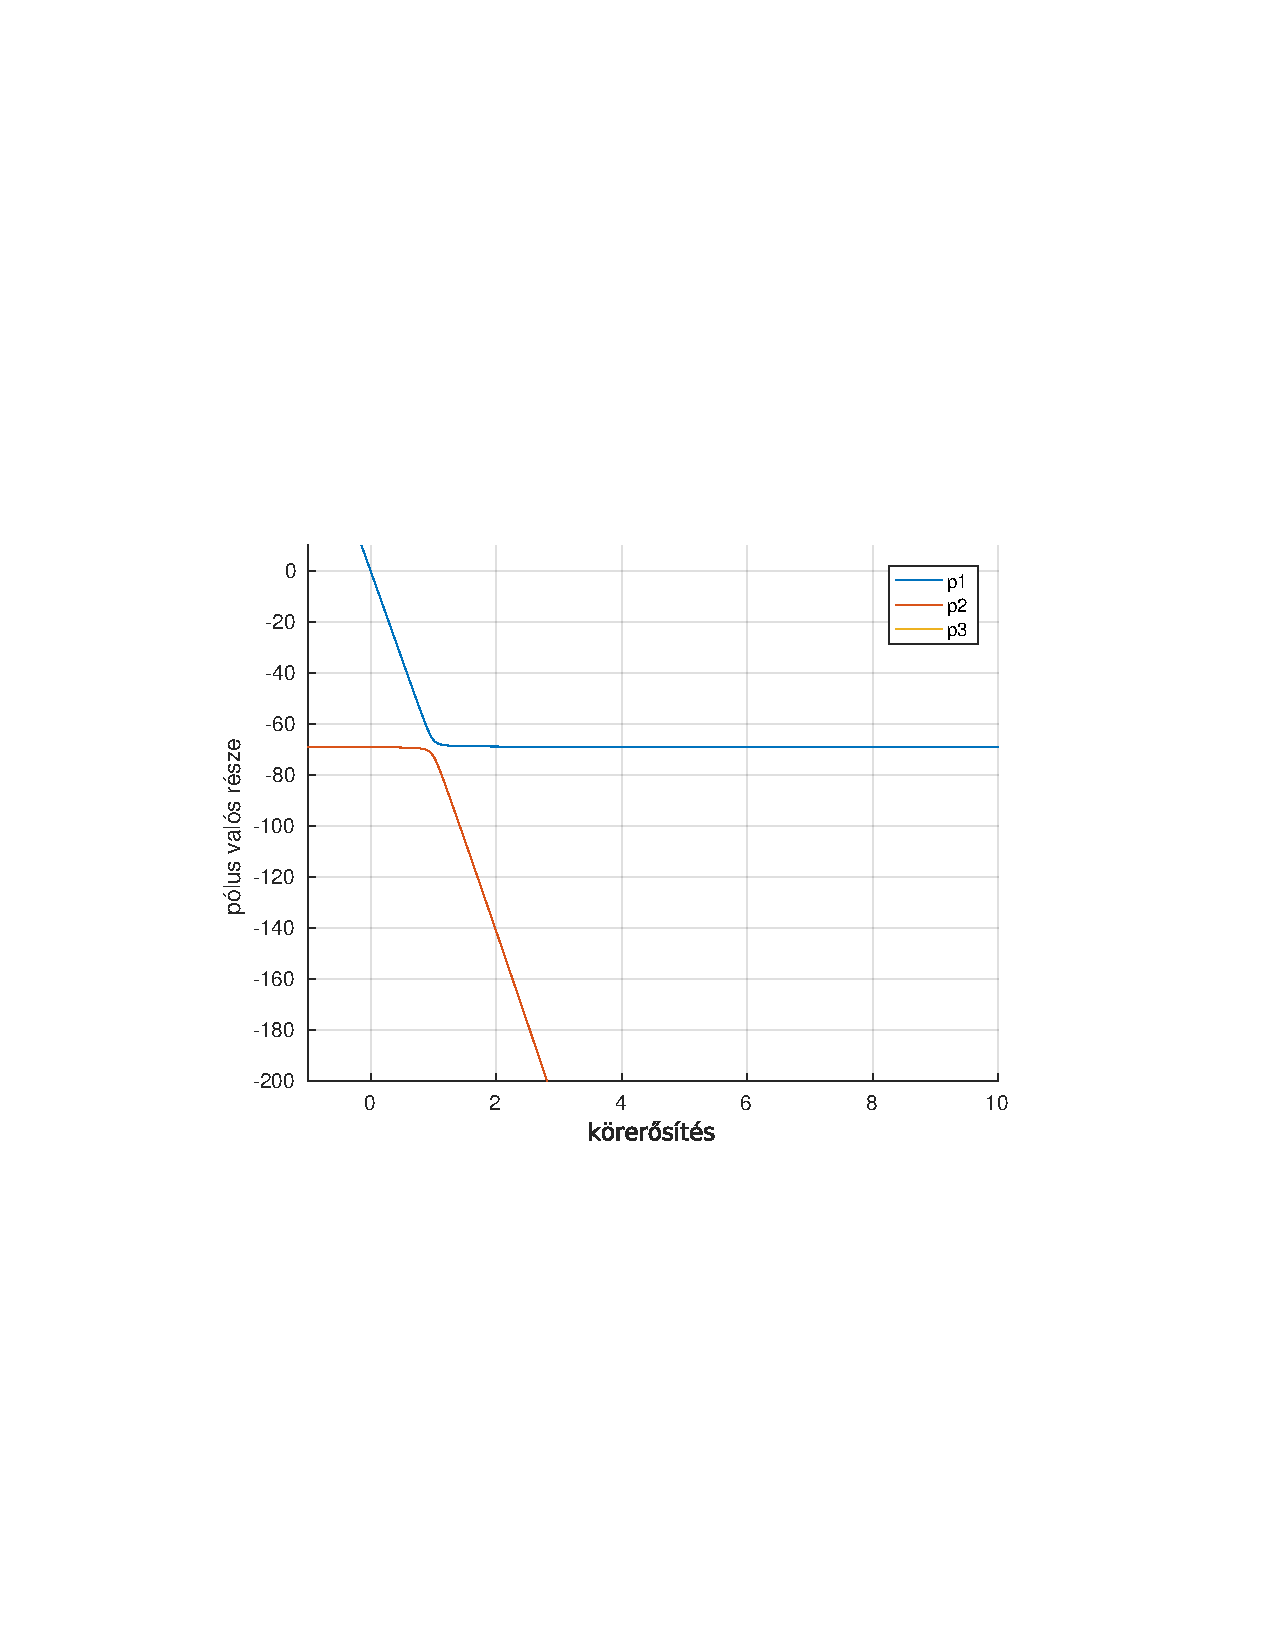
\includegraphics[width=\linewidth, trim=90 240 100 242, clip]{polus-big}
		\caption{0 körüli $P$-k}
	\end{subfigure}
	\caption{Pólusok valós része a körerősítés függvényében}
	\label{fig:poles}
\end{figure}

%}}}

%{{{ Megadott körerősítés esetén Bode-diagram és fázistartalék
\subsection{Megadott körerősítés esetén Bode-diagram és fázistartalék}

Válasszuk a körerősítést $P=\vartheta_2 = 4,063$-re.
Ennek a rendszernek a Bode-diagramját mutatja \aref{fig:bode}. ábra.
A \verb|margin| függvényt használva megkapjuk a fázistartalékot,
ami $\varphi_\text{m}=60^\circ$.

\begin{figure}[H]
	\centering
	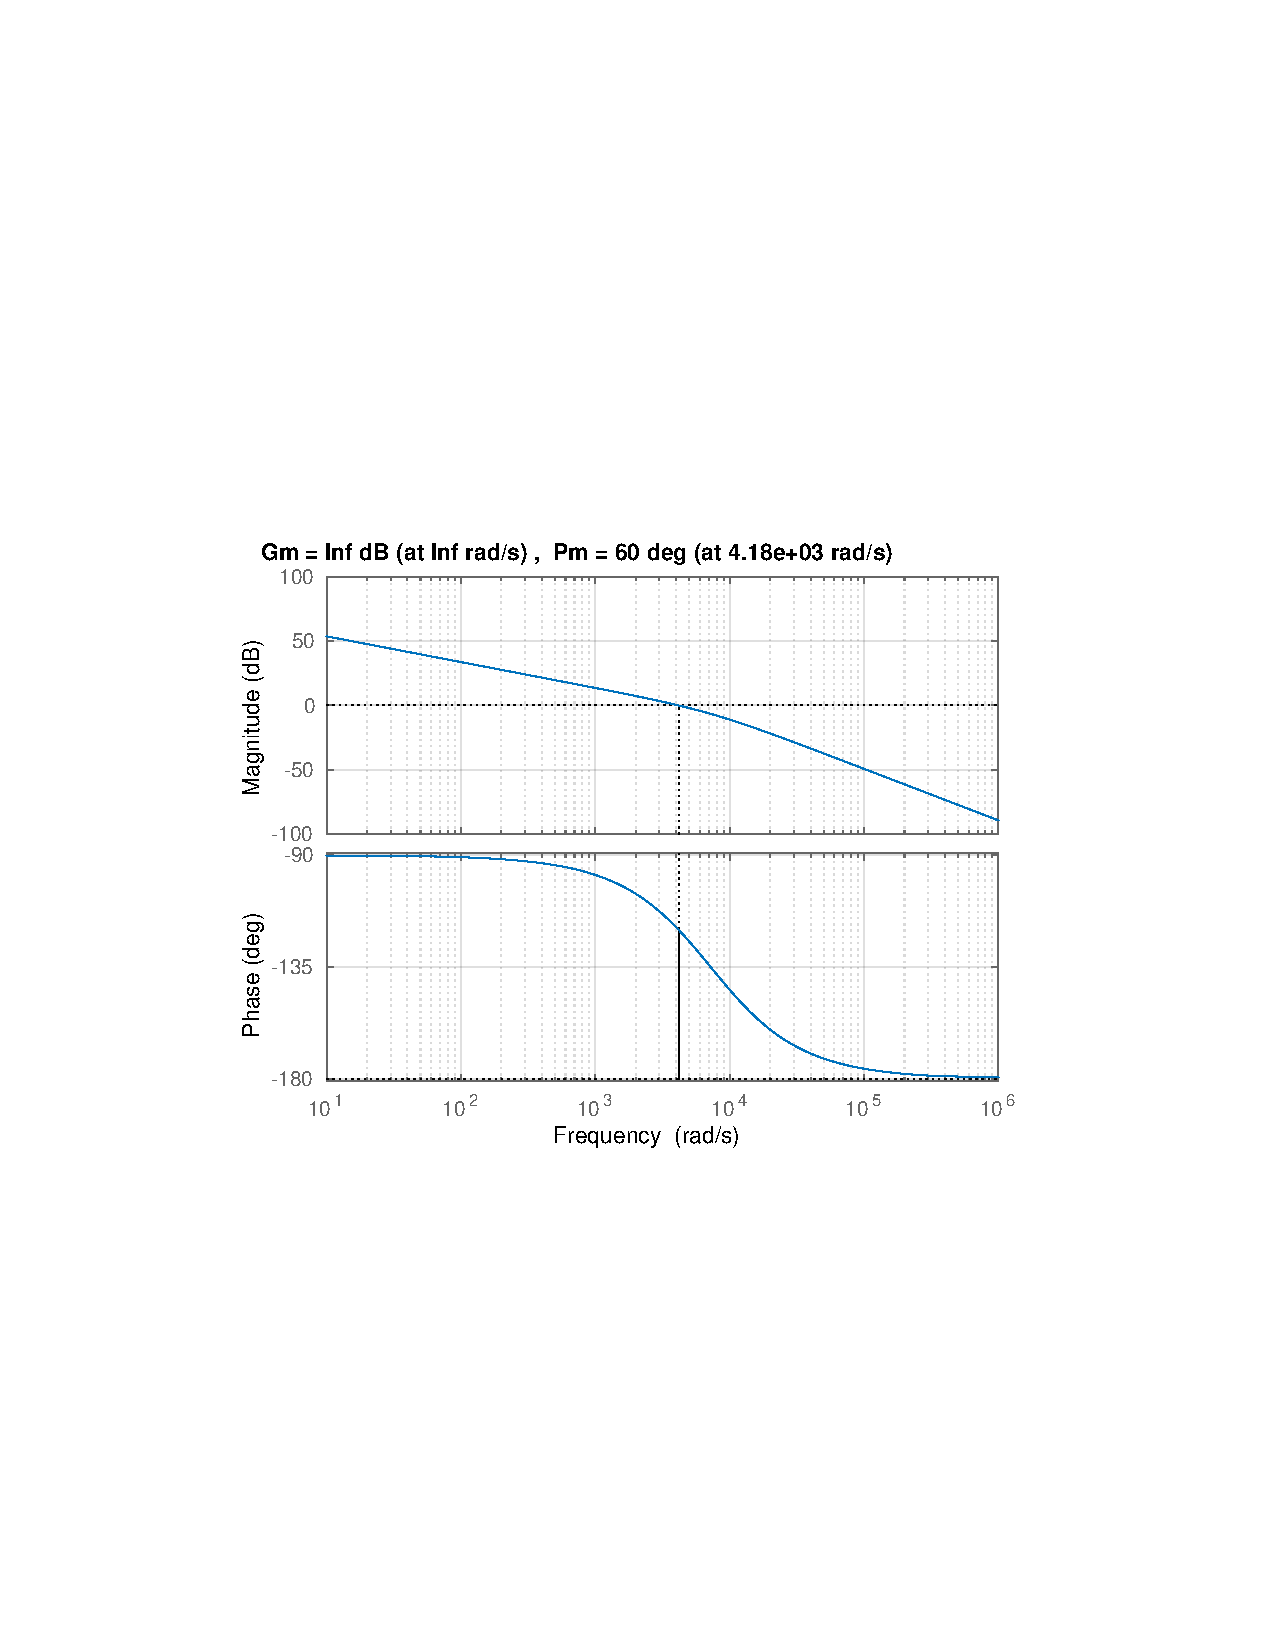
\includegraphics[width=.8\textwidth, trim=100 240 80 252, clip]{bode}
	\caption{Szabályozási kör Bode-diagramja}
	\label{fig:bode}
\end{figure}

%}}}

%{{{ Súlyfüggvény
\subsection{Súlyfüggvény}

A súlyfüggvényt könnyen kirajzolhatjuk az \verb|impulse| függvénnyel.
Az alapjel a névleges szögsebesség fele, vagyis
\begin{equation}
	\Omega_0 = \frac{\omega_\text{n}}{2} = 231.96~\frac{\text{rad}}{\text{s}}.
\end{equation}

\begin{figure}[H]
	\centering
	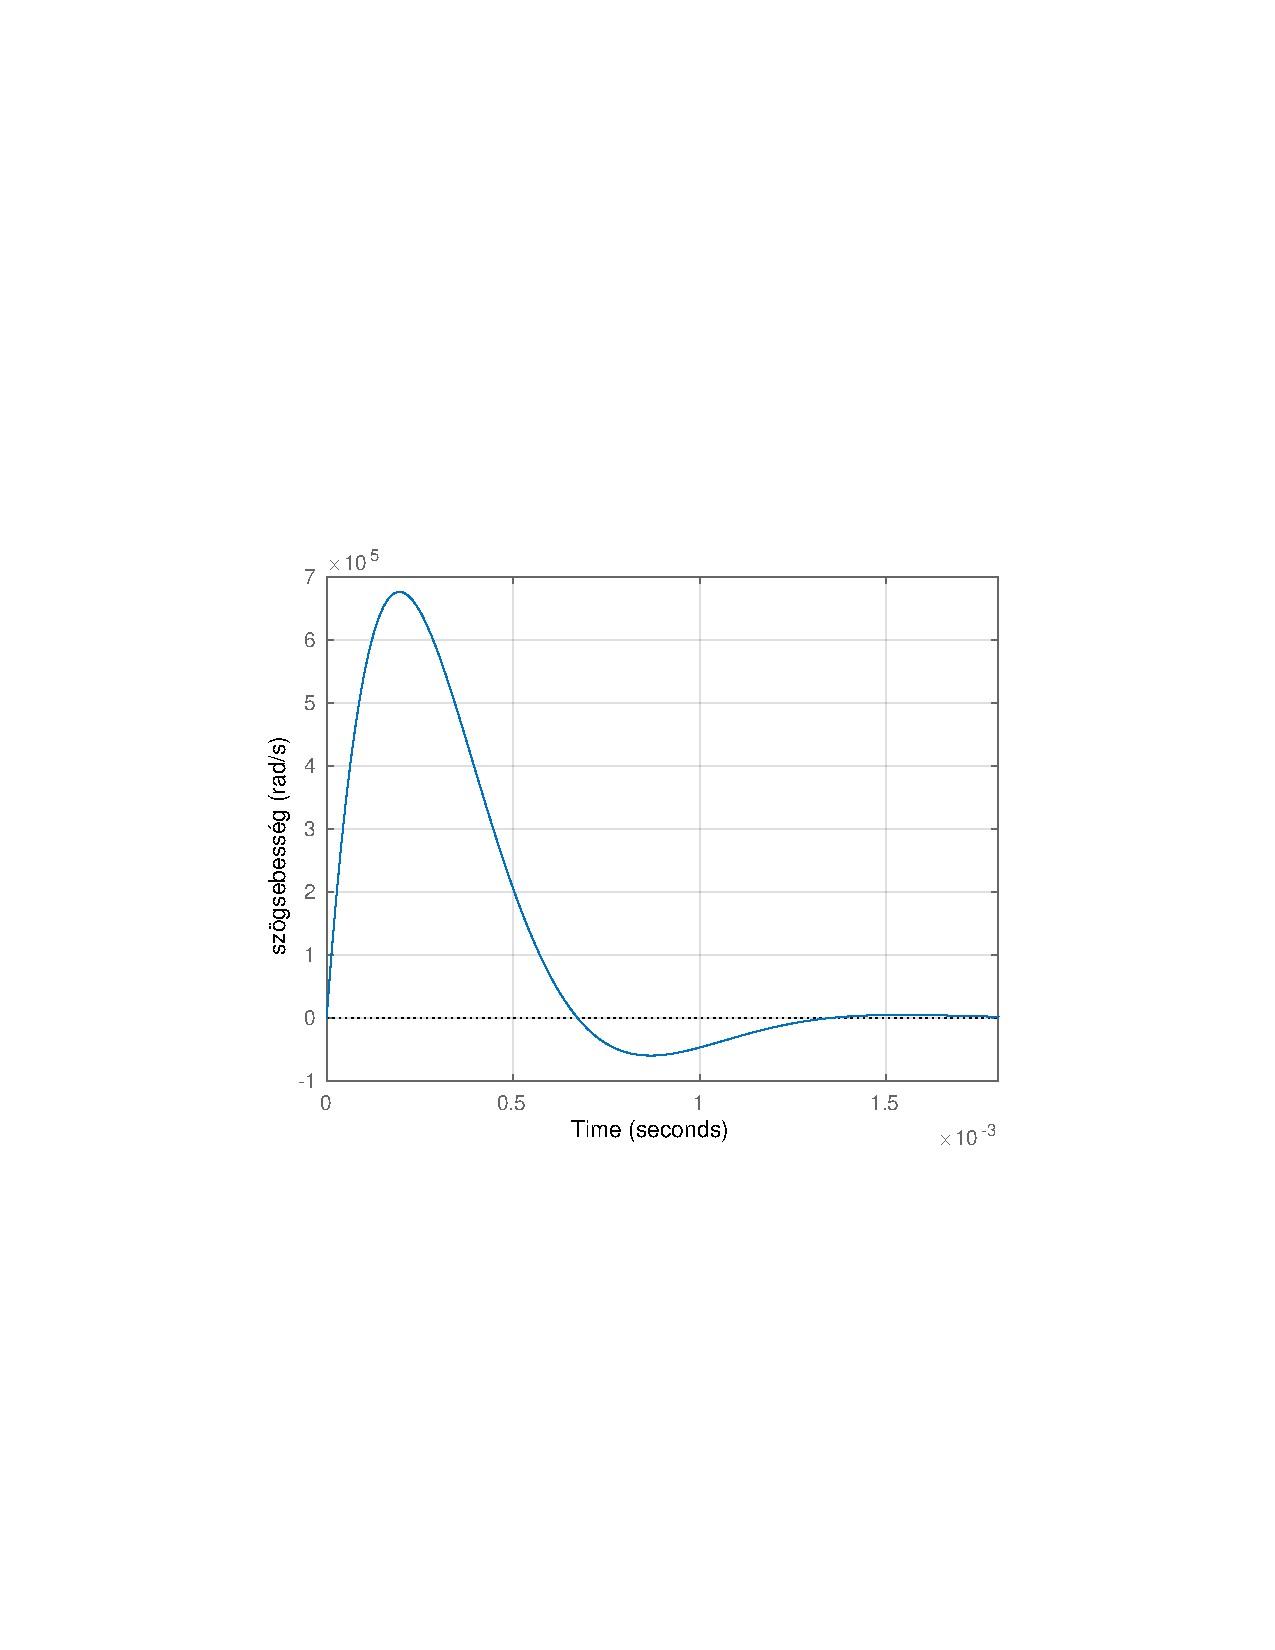
\includegraphics[width=.7\textwidth, trim=100 240 80 252, clip]{impulse}
	\caption{A zárt szabályozási kör impulzusválasza}
	\label{fig:impulse}
\end{figure}

%}}}

%{{{ Átmeneti függvény
\subsection{Átmeneti függvény}

Az átmeneti függvényt a \verb|step| függvény adja meg.
Az alapjel itt is a névleges szögsebesség fele.

\begin{figure}[H]
	\centering
	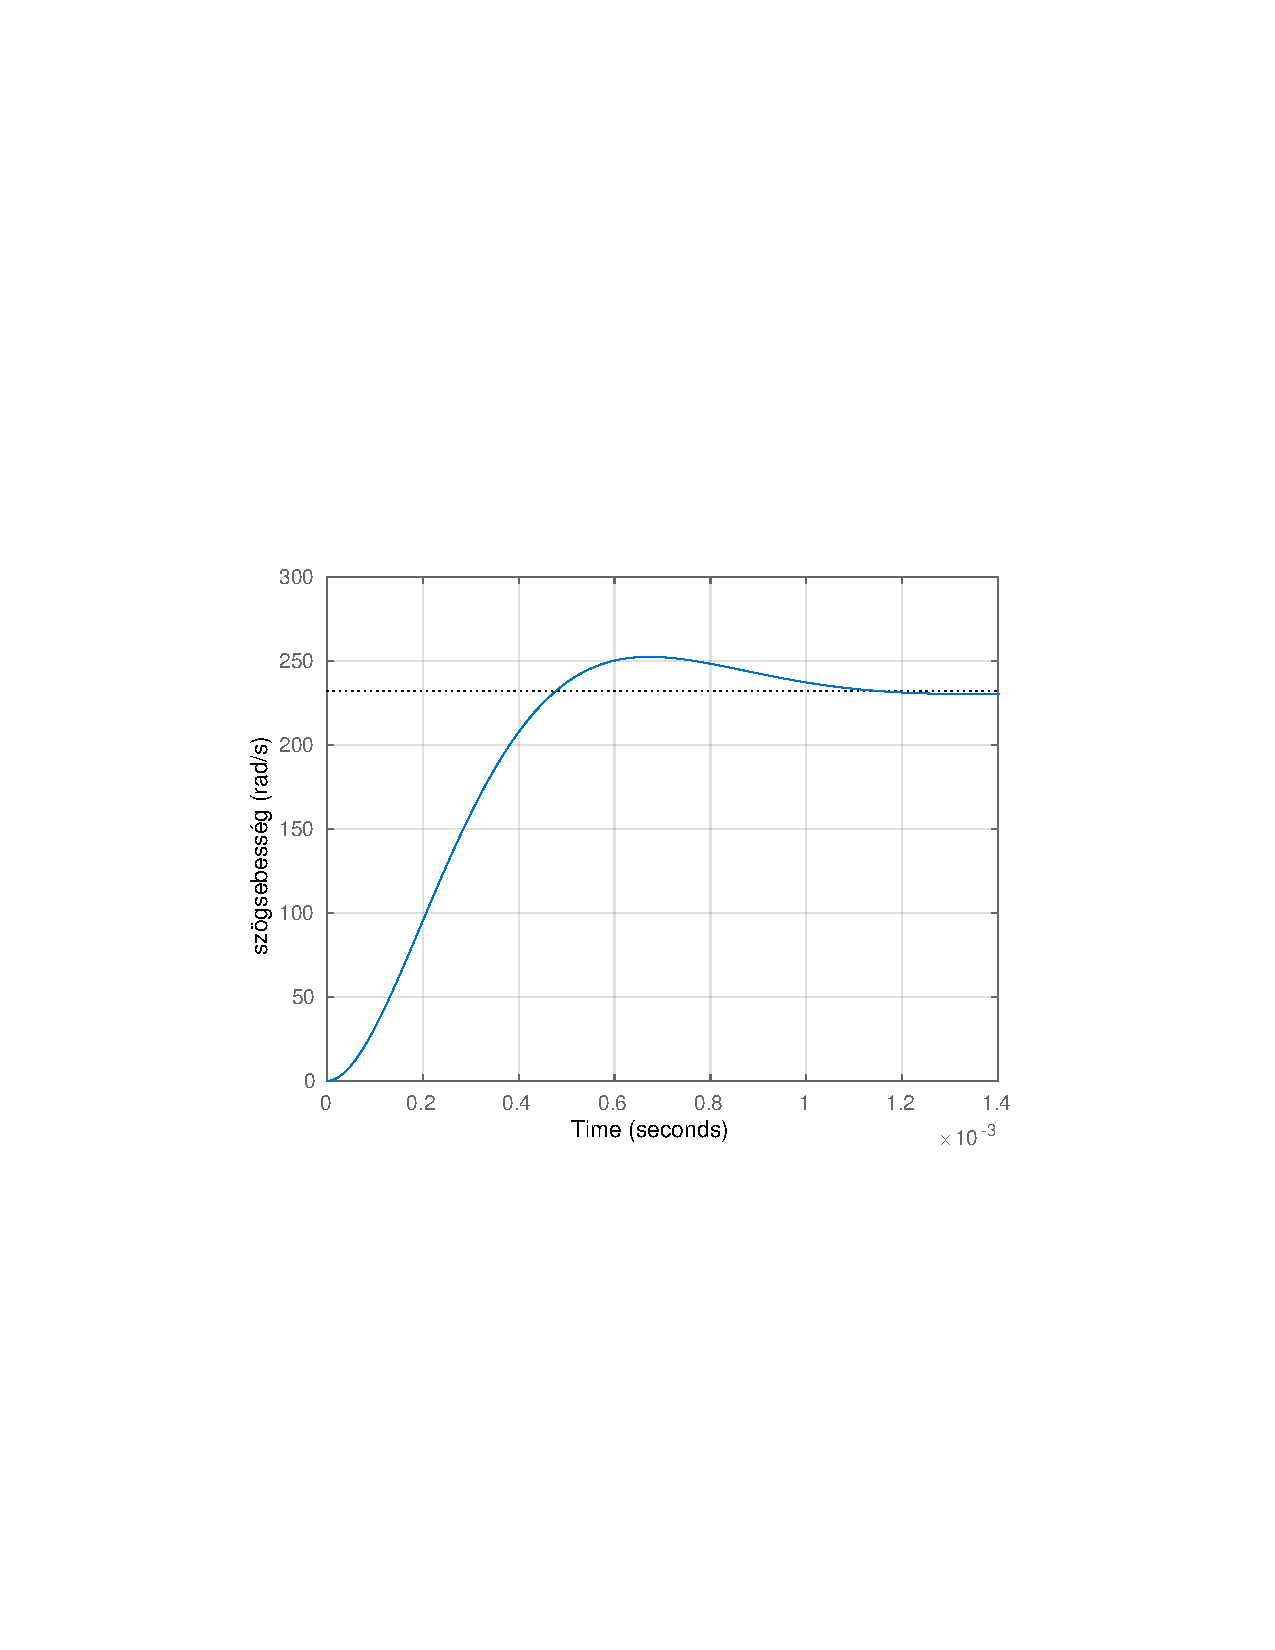
\includegraphics[width=.7\textwidth, trim=100 240 80 252, clip]{step}
	\caption{A zárt szabályozási kör átmeneti függvénye}
	\label{fig:step}
\end{figure}

%}}}
